\documentclass[12pt,a4paper,oneside]{article}
\input{environment}
\usepackage{longtable}
\usepackage[dutch]{babel}
\usepackage{titling,enumitem}
\usepackage{graphicx}
\usepackage{tikz}
\usepackage{a4wide}
\usepackage{amsmath}
\usepackage{amssymb}
\usepackage{rotating}
\usepackage{listings}
\usepackage{float}
\usepackage{color}
\usepackage{fancyhdr}
\usepackage{lastpage}
% packages
\usepackage[T1]{fontenc}
\usepackage[margin=3cm]{geometry}
\usepackage{array, xcolor}
\usepackage{titling}
\usepackage{blindtext}
\usepackage{pdfpages}
% rules
\definecolor{lightgray}{gray}{0.8}
\newcolumntype{L}{>{\raggedleft}p{0.50\textwidth}}
\newcolumntype{R}{p{0.8\textwidth}}
\newcommand\VRule{\color{lightgray}\vrule width 0.5pt}
%%%%%%%%%%%%TABULAR SHIT%%%%%%%%%%%%%%%%%%
\usepackage{color, colortbl}
\definecolor{Gray}{gray}{0.9}
%%%%%%%%%%%%%%%%%%%%%%%%%%%%%%%%%%%%%%%%
%SECTION SHIT
\renewcommand*{\thesubsubsection}{\Alph{section}}
\definecolor{dkgreen}{rgb}{0,0.6,0}
\definecolor{gray}{rgb}{0.5,0.5,0.5}
\definecolor{mauve}{rgb}{0.58,0,0.82}
 
\lstset{ %
  language=PYTHON,                
  basicstyle=\footnotesize,           
  numbers=left,                  
  numberstyle=\tiny\color{gray},  
  stepnumber=2,                        
  numbersep=5pt,                  
  backgroundcolor=\color{white},      
  showspaces=false,               
  showstringspaces=false,        
  showtabs=false,                 
  frame=single,                   
  rulecolor=\color{black},        
  tabsize=2,                      
  captionpos=b,                   
  breaklines=true,                
  breakatwhitespace=false,        
  title=\lstname,                                                  
  keywordstyle=\color{blue},          
  commentstyle=\color{dkgreen},       
  stringstyle=\color{mauve},         
  escapeinside={\%*}{*)},            
  morekeywords={*,...},              
  deletekeywords={...}              
}
\begin{document}
\includepdf[pages={1}]{titlepage.pdf}
\pagestyle{fancy}
\fancyhf{}
\fancyhead[R]{Groep 16}
\fancyhead[L]{SO2: Behoeftenanalyse en Architectuur}
\fancyfoot[L]{\small Vakgroep Informatietechnologie \\ Gaston Crommenlaan 8, bus 201, B - 9050 Gent \\ www.intec.UGent.be}
\fancyfoot[R]{\small \thepage / \pageref{LastPage}}
\section*{Behoeftenanalyse}
\section{UML-use case diagram}
\begin{figure}[H]
  \begin{center}
    \includegraphics[width=\textwidth]{use_case_diagram2-eps-converted-to.pdf}
    \caption{Use case diagram}
    \label{graph:graph1}
  \end{center}
\end{figure}
\section{Use-case beschrijving}
\setcounter{section}{1}
\subsubsection{Use-case 1}
\begin{uc}{De security waarschuwen}

    \begin{uc-mss}{De security wordt op de hoogte gebracht}
    \item De bril maakt een foto.
\item De bril bepaalt de huidige locatie voor het attribuut locatie in Foto.
    \item De bril maakt verbinding met de brillen van de security.
    \item De bril verzend een push-melding met de Foto en de Locatie.
\item Scenario be\"eindigd, postconditie geldt vanaf nu.
    \end{uc-mss}

    \begin{uc-ext}

     \begin{uc-fail}{2}{De locatie van de gebruiker is onbekend}
        \item Zet locatie op onbekend. 
	\item Ga naar MSS stap 3.
        \end{uc-fail}

        \begin{uc-fail}{3}{Er kan geen verbinding worden gemaakt met de security}
        \item In plaats van met de security maakt de bril verbinding met de politie.
        \item Ga naar MSS stap 4.
        \end{uc-fail}

     \end{uc-ext}

    \begin{uc-pre}
    \item De camera en de GPS-ontvanger zijn actief.
    \end{uc-pre}

    \begin{uc-post}
    \item De bril van de security krijgt een pushnotificatie van het incident.    \end{uc-post}

    \begin{uc-trig}
    \item De gebruiker meldt een incident met het spraakcommando `incident melden'.
    \end{uc-trig}

\end{uc}
\setcounter{section}{2}
\subsubsection{Use-case 2}
\begin{uc}{Webshop}

    \begin{uc-mss}{}
    \item De bril ontvangt via bluetooth een afbeelding van een kledingstuk.
    \item De camera zoekt naar het silhouet van een persoon.
    \item De afbeelding wordt geprojecteerd op de bril.
    \item De camera maakt foto's en analyseert de beelden.
    \item Aan de hand van de foto's berekent de bril de afmetingen van de gebruiker.
    \item Met de spraakcommando's 'next' en 'previous' kan de gebruiker het vorige of het volgende kledingstuk passen uit zijn/haar verlanglijstje.
    \item Met het commando 'buy' stuurt de bril een signaal naar de pc om het huidige kledingstuk in het winkelmandje te plaatsen in de juiste maat.
\item Scenario be\"eindigd, postconditie geldt vanaf nu.
    \end{uc-mss}

    \begin{uc-ext}

        \begin{uc-fail}{2}{De camera herkent geen silhouet (na een bepaalde tijd)}
        \item Er verschijnt een boodschap "Ga voor de spiegel staan".
        \item Met het commando "search again"\, begint de camera opnieuw te zoeken.
        \end{uc-fail}
        
        \begin{uc-fail}{7}{De bluetooth verbinding is verbroken}
        \item Er verschijnt een foutboodschap.
        \end{uc-fail}

    \end{uc-ext}

    \begin{uc-pre}
    \item Bluetooth is ingeschakeld en er is een connectie met een pc.
    \end{uc-pre}

    \begin{uc-post}
    \item De gebruiker heeft een aantal kledingstukken gepast en eventueel besteld.
    \end{uc-post}

    \begin{uc-trig}
    \item De gebruiker stuurt via de pc een commando naar de bril.
    \end{uc-trig}

\end{uc}
\setcounter{section}{3}
\subsubsection{Use-case 3}
\begin{uc}{Geavanceerde navigatie (Indoor GPS)}

    \begin{uc-mss}{Bestemming instellen}
    \item De gebruiker stelt een bestemming in.
    \item De route wordt door de backend berekend.
    \item De kaart met route wordt op de bril geprojecteerd.
    \item De gebruiker loopt door het gebouw.
    \item De bril stuurt foto's door om de huidige locatie te updaten.
    \item De gebruiker loopt tot als hij zijn bestemming bereikt heeft.
\item Scenario be\"eindigd, postconditie geldt vanaf nu.
    \end{uc-mss}

    \begin{uc-ext}

        \begin{uc-fail}{1}{De bestemming bestaat niet of wordt niet herkend}
        \item Geef een foutmelding en laat de gebruiker opnieuw proberen.
        \end{uc-fail}
        
        \begin{uc-fail}{2}{Er is geen verbinding met het systeem}
        \item Toon een foutmelding. 
        \item Probeer opnieuw als de gebruiker aangeeft dat er verbinding met het internet is.
        \end{uc-fail}
        
        \begin{uc-fail}{4}{De gebruiker loopt verkeerd.}
        \item Herbereken de route.
        \item Ga naar MSS stap 3.
        \end{uc-fail}

    \end{uc-ext}

    \begin{uc-pre}
    \item De GPS functie en camera zijn actief.
    \item De bril heeft verbinding met het backendsysteem.
    \item De backend weet waar de gebruiker zich bevindt.
    \end{uc-pre}

    \begin{uc-post}
    \item De gebruiker heeft zijn bestemming bereikt.
    \end{uc-post}

    \begin{uc-trig}
    \item De gebruiker drukt op 'Bestemming instellen'.
    \end{uc-trig}

\end{uc}
\setcounter{section}{4}
\subsubsection{Use-case 4}
\begin{uc}{Augmented Reality overlay}

    \begin{uc-mss}{Object krijgt een overlay}
	\item De bril scant de omgeving naar objecten.
	\item De bril stuurt gevonden objecten naar het backendsysteem.
	\item Het object wordt herkend door het backendsysteem.
	\item De overlay-informatie wordt ontvangen in de bril.
	\item De bril geeft de extra informatie over het object weer in een overlay.
	\item De bril geeft een optie om de huidige informatie te verbeteren of nieuwe informatie toe te voegen.
	\item Scenario be\"eindigd, postconditie geldt vanaf nu.
    \end{uc-mss}

    \begin{uc-ext}

		\begin{uc-fail}{2,4}{Er is geen verbinding meer met het systeem}
		\item Toon een foutmelding.
		\item Probeer automatisch of op vraag van de gebruiker opnieuw te connecteren met het internet.
		\end{uc-fail}		
		\begin{uc-fail}{3}{Het object is niet opgenomen in de database}
		\item Toon een waarschuwing.
		\item Geef de gebruiker de mogelijkheid om dit object toe te voegen.
		\end{uc-fail}		
		\begin{uc-fail}{5}{Er is geen extra informatie beschikbaar}
		\item Toon een waarschuwing.
		\end{uc-fail}

    \end{uc-ext}

    \begin{uc-pre}
	\item De camera is actief.
	\item De bril heeft verbinding met het backendsysteem.
    \end{uc-pre}

    \begin{uc-post}
	\item Alle objecten hebben een correcte overlay.
    \end{uc-post}

    \begin{uc-trig}
	\item De AR-applicatie wordt opgestart.
    \end{uc-trig}

\end{uc}
\section*{I	\;\;\;Architectuur: klassendiagram}
\setcounter{section}{0}
\section{Projectbeschrijving}
Een eerste functie van de bril is het \textbf{binnenshuis navigeren}, waardoor de route als overlay op de bril wordt \textbf{geprojecteerd}. Omdat er geen GPS-ontvangst mogelijk is, wordt er op regelmatige tijdstippen beelden van de bril doorgestuurd. Door vergelijking van opgeslagen beelden kan de locatie van de gebruiker bepaald worden. De bril kan ook in leermodus geschakeld worden, waarbij de videobeelden van de bril doorgestuurd worden, en de gebruiker kan aangeven waar hij zich bevindt.
\\
\\
Een tweede mogelijkheid van de bril bestaat erin dat de beelden van de bril constant \textbf{doorgestuurd} en geanalyseerd worden door een back-end systeem om \textbf{voorwerpen en personen te herkennen}. Hierbij wordt wordt gebruik gemaakt van een gegevensdatabank. De meta-data van herkende voorwerpen of personen wordt opgehaald uit de databank en naar de gebruiker doorgestuurd. De gebruiker kan desgewenst bijkomende informatie opvragen. Ook deze applicatie beschikt over een leermodus, zodat gebruikers meta-informatie kunnen toevoegen of bewerken in de databank.
\\
\\
Een derde mogelijkheid heeft te maken met online shopping. Wanneer de gebruiker doorheen de webwinkel navigeert en een kledingstuk aanklikt, kan hij zichzelf zien met deze kleren aan. Het kledingstuk wordt als overlay \textbf{geprojecteerd} op je bril zodat het lijkt alsof je de kleren echt aan hebt. Terwijl de gebruiker voor de spiegel staat meet de bril de maten op en vergelijkt die met de matentabel, zo weet je ook onmiddellijk welke maat je zal nodig hebben.
\\
\\
Tenslotte helpt de bril mee aan de algemene veiligheid. Wanneer de gebruiker zich bevindt op een publieke plaats, wordt er automatisch verbinding gemaakt met de brillen van de security. Dit kan bijvoorbeeld een station, een winkel of een nachtclub zijn. Wanneer de gebruiker iets verdacht opmerkt, dit kan bijvoorbeeld een gevecht zijn, kan de gebruiker het incident rapporteren en wordt de security op de hoogte gebracht. Er wordt een foto getrokken en de locatie wordt bepaald. Dit kan met behulp van use case 1: \textbf{binnenshuis navigeren}. Zij worden doorgestuurd naar de security. Op die manier is er ook onmiddellijk bewijs tegen de daders.
\\
\\
De belangrijkste common core functies van onze usecases zijn dus projectie, het doorsturen van beelden en de Indoor GPS.
\newpage
\section{Klassenlijst}
\begin{longtable}{|l|p{6cm}|p{5cm}|}
\hline\rowcolor{Gray}
\textbf{Klassenaam} & \textbf{Attributen/Operaties}& \textbf{Opmerkingen}\\ 
\hline
Gebruiker&\vspace*{-10mm}
\begin{itemize}[parsep=-2pt,leftmargin=0.3cm]
\item \texttt{private Account account}
\item \texttt{public void setAccount(Account account)} 
\item \texttt{public Multimedia maakNieuweVideo()} 
\item \texttt{public void verbindApparaat()}
\item \texttt{public void startNavigatie()
\item\texttt{public void herkenObjecten()}}\vspace*{-6mm} 
\end{itemize}&Kan m.b.v. zijn account ge\"identificeerd worden.\\
\hline
Account&\vspace*{-10mm}
\begin{itemize}[parsep=-2pt,leftmargin=0.3cm]
\item \texttt{private String naam}
\item \texttt{private String voornaam} 
\item \texttt{private String email} 
\item \texttt{public String getNaam()}
\item \texttt{public String getVoornaam()}
\item \texttt{public String getEmail()}
\item \texttt{public void setNaam(String naam)}
\item \texttt{public void setVoornaam(String voornaam)}
\item \texttt{public void setEmail(String email)}\vspace*{-6mm} 
\end{itemize}&Uniek per gebruiker.\\
\hline
GUI &\vspace*{-10mm}\begin{itemize}[parsep=-2pt,leftmargin=0.3cm] 
\item \texttt{public void projecteer(Multimedia media)} \vspace*{-6mm} 
\end{itemize}& Op deze manier kunnen er allerlei dingen geprojecteerd worden op de bril.\\
\hline
Locatie&\vspace*{-10mm}\begin{itemize}[parsep=-2pt,leftmargin=0.3cm]
\item \texttt{private float latitude} 
\item \texttt{private float longitude}
\item \texttt{private String address}
\item \texttt{public void setLatitude(float latitude)}
\item \texttt{public void setLongitude(float longitude)}
\item \texttt{public void setAddress(String adres)}
\item \texttt{public float getLatitude()}
\item \texttt{public float getLongitude()}
\item \texttt{public float getAddress()}
\vspace*{-6mm} 
\end{itemize}&\\
\hline
Tijdstip&\vspace*{-10mm}\begin{itemize}[parsep=-2pt,leftmargin=0.3cm]
\item \texttt{private int dag,maand,jaar} 
\item \texttt{private int uur, minuten, seconden} 
\item \texttt{public void setDatum(int dag, int maand, int jaar)}
\item \texttt{public void setUur(int uur, int minuten, int seconden)}
\item \texttt{public int[] getDatum()}
\item \texttt{public int[] getUur()}
\vspace*{-6mm} \end{itemize}&\\
\hline
Camera&\vspace*{-10mm}\begin{itemize}[parsep=-2pt,leftmargin=0.3cm]
\item \texttt{public Foto maakFoto()} 
\item \texttt{public Video maakVideo()}\vspace*{-6mm} \end{itemize}&\\
\hline
Video&\vspace*{-10mm}\begin{itemize}[parsep=-2pt,leftmargin=0.3cm]
\item \texttt{private Tijdstip tijdstip} 
\item \texttt{private Locatie locatie}\vspace*{-6mm} 
\end{itemize}&\\
\hline
Foto&\vspace*{-10mm}\begin{itemize}[parsep=-2pt,leftmargin=0.3cm]
\item \texttt{private Tijdstip tijdstip} 
\item \texttt{private Locatie locatie}\vspace*{-6mm} 
\end{itemize}&\\
\hline
BrilConnectie&\vspace*{-10mm}\begin{itemize}[parsep=-2pt,leftmargin=0.3cm]
\item \texttt{private Account account1} 
\item \texttt{private Account account2} 
\item \texttt{public void maakVerbinding()}\vspace*{-6mm} 
\end{itemize}&Verbinding tussen 2 brillen.\\
\hline
Apparaatconnectie&\vspace*{-10mm}\begin{itemize}[parsep=-2pt,leftmargin=0.3cm] \item \texttt{private String deviceID} \vspace*{-6mm} 
\end{itemize}&Bv een bluetoothconnectie tussen de bril en een computer.\\
\hline
AudioInput&\vspace*{-10mm}\begin{itemize}[parsep=-2pt,leftmargin=0.3cm] 
\item \texttt{public void listen()} \vspace*{-6mm} 
\end{itemize}&Neemt de gesproken boodschap op en geeft ze mee aan de VoiceCommandRecognizer.\\
\hline
VoiceCommandRecognizer&\vspace*{-10mm}\begin{itemize}[parsep=-2pt,leftmargin=0.3cm] 
\item \texttt{public void recognize(AudioInput audio)} 
\item \texttt{public void voerCommandoUit(String commando)} \vspace*{-6mm} 
\end{itemize}&Verwerkt de gesproken commando's van de gebruiker.\\
\hline
GPSApplicatie&\vspace*{-10mm}\begin{itemize}[parsep=-2pt,leftmargin=0.3cm] 
\item \texttt{private Locatie start} 
\item \texttt{private Locatie bestemming} 
\item \texttt{private List<Locatie> tussenpunten} 
\item \texttt{public void herbereken()}  
\item \texttt{public String getVolgendeInstructie()} 
\item \texttt{public void setStart(Locatie locatie)}
\item \texttt{public void setBestemming(Locatie locatie)()}
\vspace*{-6mm} 
\end{itemize}&Wanneer de gebruiker de volgende locatie in de lijst bereikt heeft, wordt \texttt{getVolgendeInstructie()} opgeroepen.\\
\hline
FotoAnalyser&\vspace*{-10mm}\begin{itemize}[parsep=-2pt,leftmargin=0.3cm]
\item \texttt{private Map<Foto, Locatie> fotos}
\item \texttt{public Locatie matchLocatie(Foto foto)} 
\item \texttt{public void bewerkFouteLocatie(Locatie locatie)}
\item \texttt{public String herkenSilhouet(Foto foto)}
\item \texttt{public String herkenObject(Foto foto)}
\item \texttt{public Array<Float> berekenMaten()}\vspace*{-6mm} 
\end{itemize}& Deze klasse analyseert en vergelijkt fotos en videobeelden met een database.\\
\hline
SecurityApplicatie &\vspace*{-10mm}\begin{itemize}[parsep=-2pt,leftmargin=0.3cm] \item \texttt{public void meldIncident(Foto foto)} \vspace*{-6mm} 
\end{itemize}& Zorgt voor het aanmaken van een nieuwe BrilConnectie en een Foto.\\
\hline
ARApplicatie &\vspace*{-10mm}\begin{itemize}[parsep=-2pt,leftmargin=0.3cm] 
\item \texttt{private FotoAnalyser analyser}
\item \texttt{private Foto object}
\item \texttt{public String herkenObject(Foto foto)} \vspace*{-6mm} 
\end{itemize}& Zorgt voor de herkenning van objecten en het aanmaken van de overlay.\\
\hline
WebshopApplicatie &\vspace*{-10mm}\begin{itemize}[parsep=-2pt,leftmargin=0.3cm] 
\item \texttt{public void run} \vspace*{-6mm} 
\end{itemize}& Zorgt voor de algemene coordinatie van de WebshopApplicatie.\\
\hline
\end{longtable}
\section{Interactiediagrammen}
\subsubsection*{Scenario 1: Security waarschuwen}
\begin{figure}[H]
  \begin{center}
    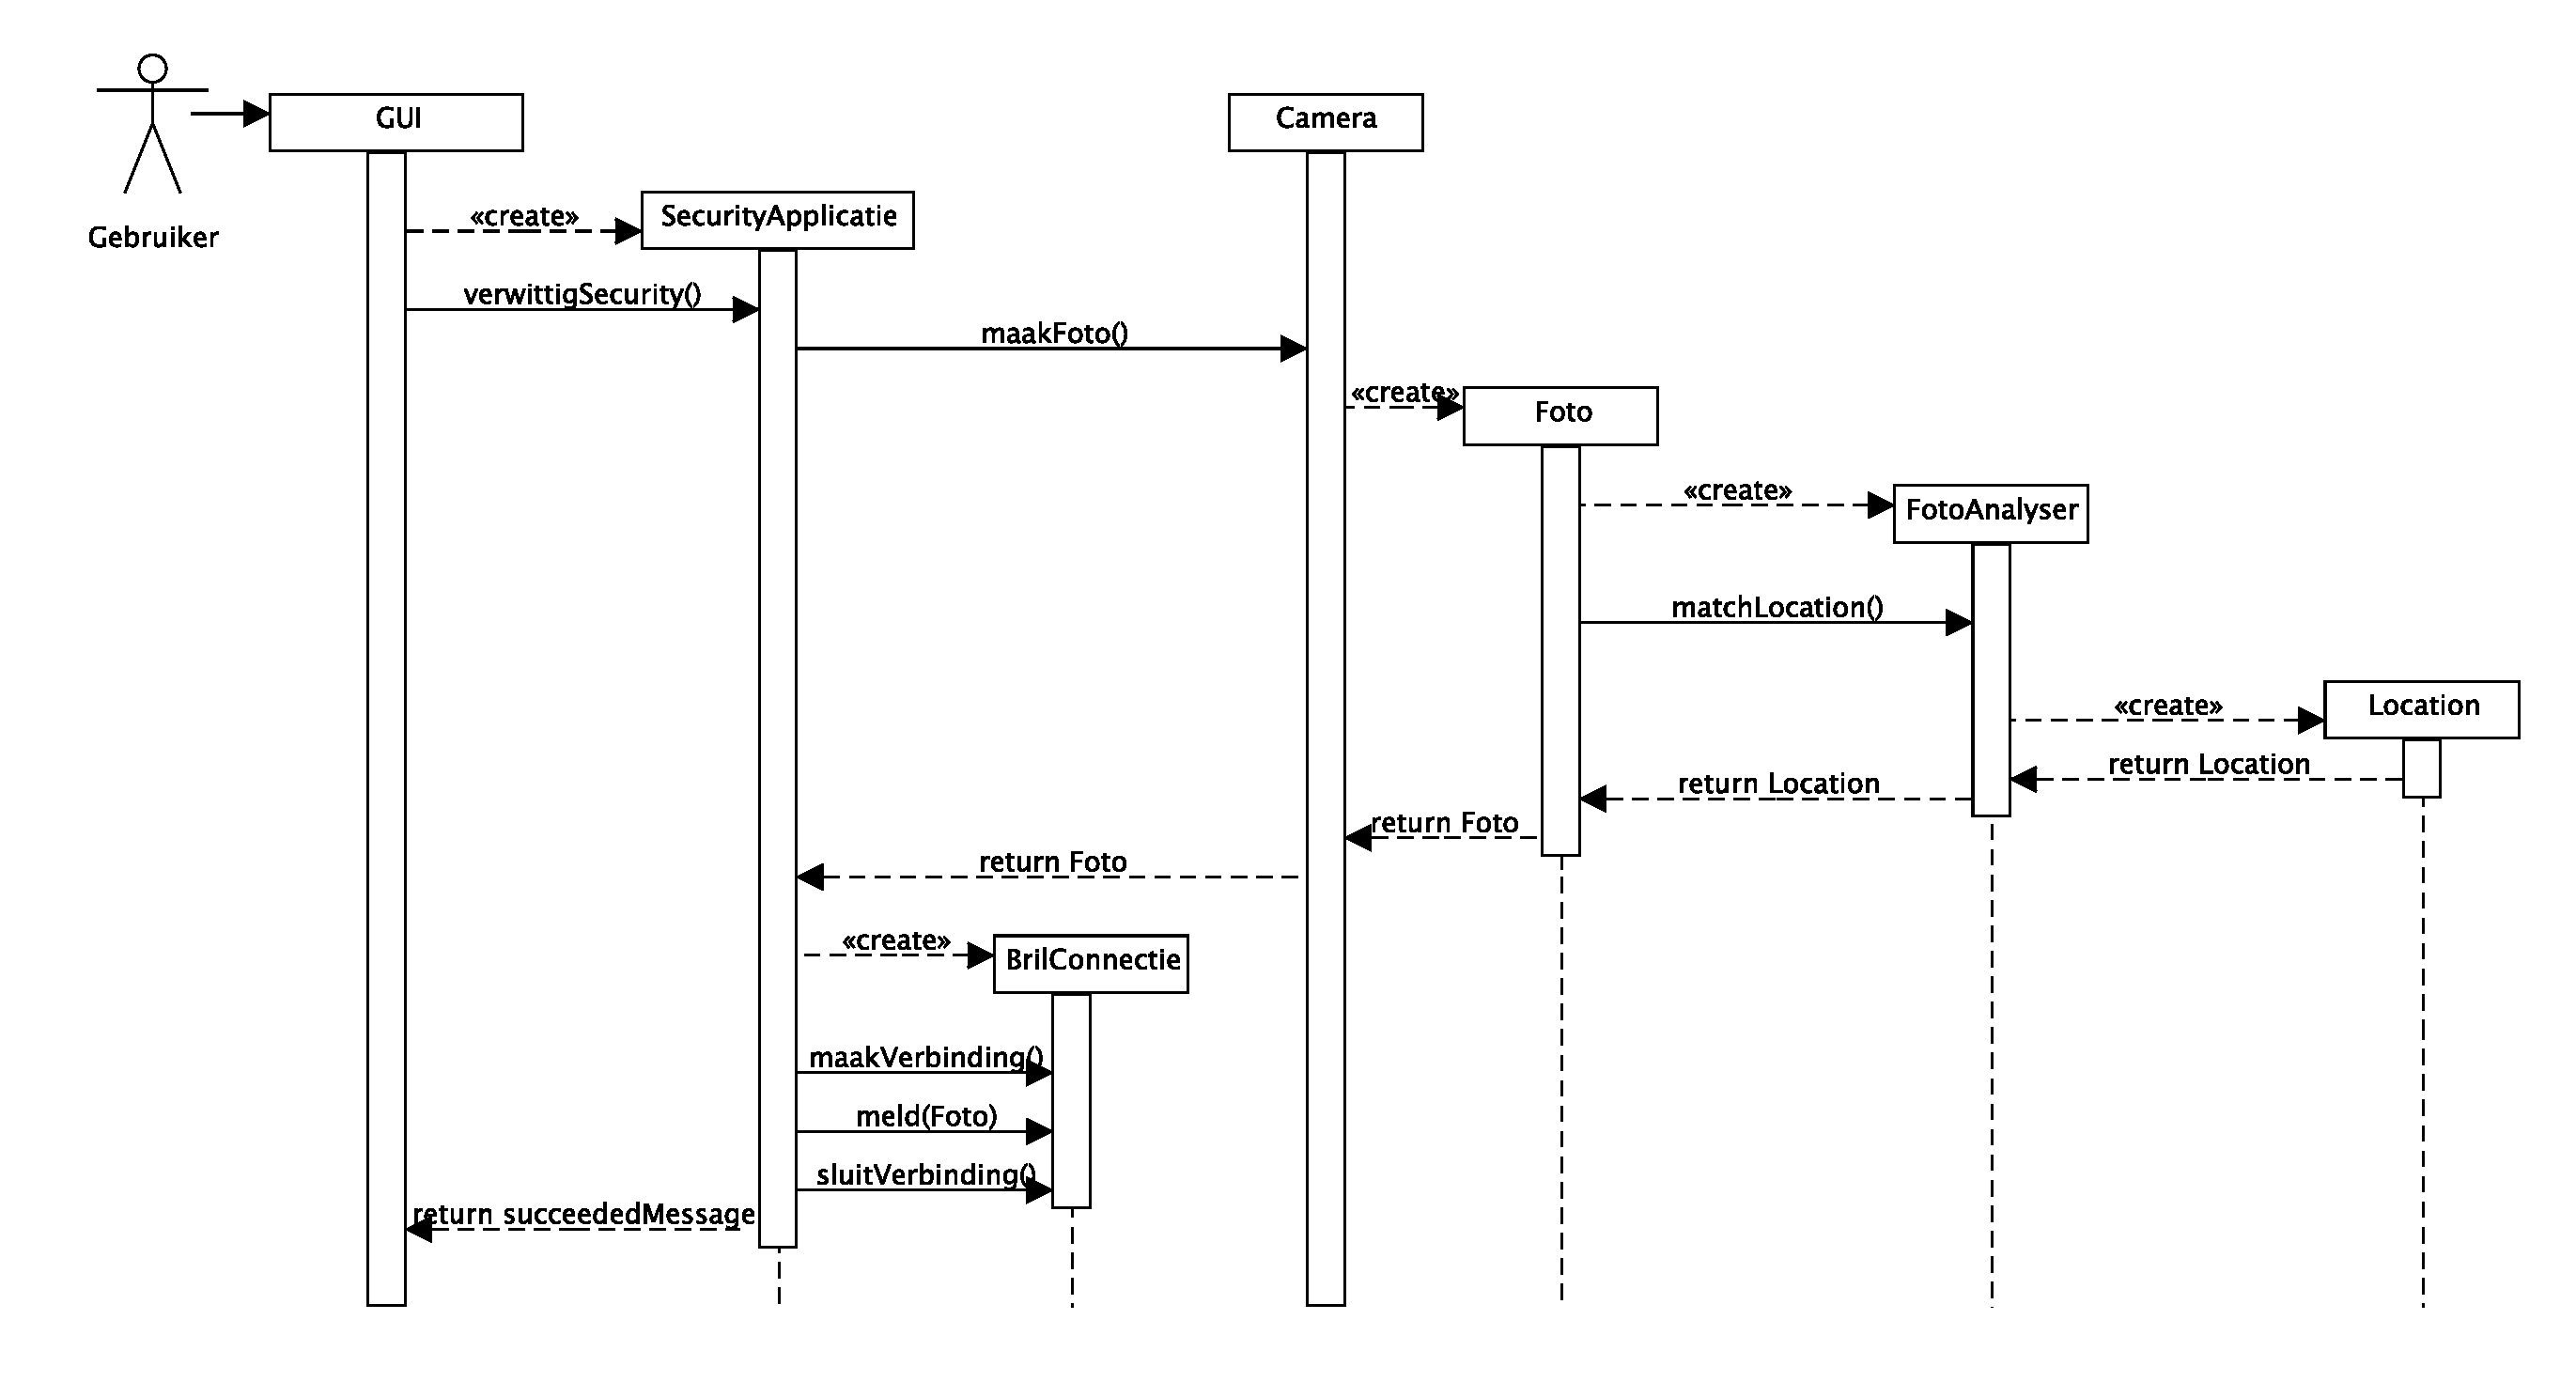
\includegraphics[scale=0.35]{sequentie_security_final.eps}
    \caption{Interactiediagram veiligheid}
    \label{graph:graph1}
  \end{center}
\end{figure}
\subsubsection*{Scenario 2: Webshop}
\begin{figure}[H]
  \begin{center}
    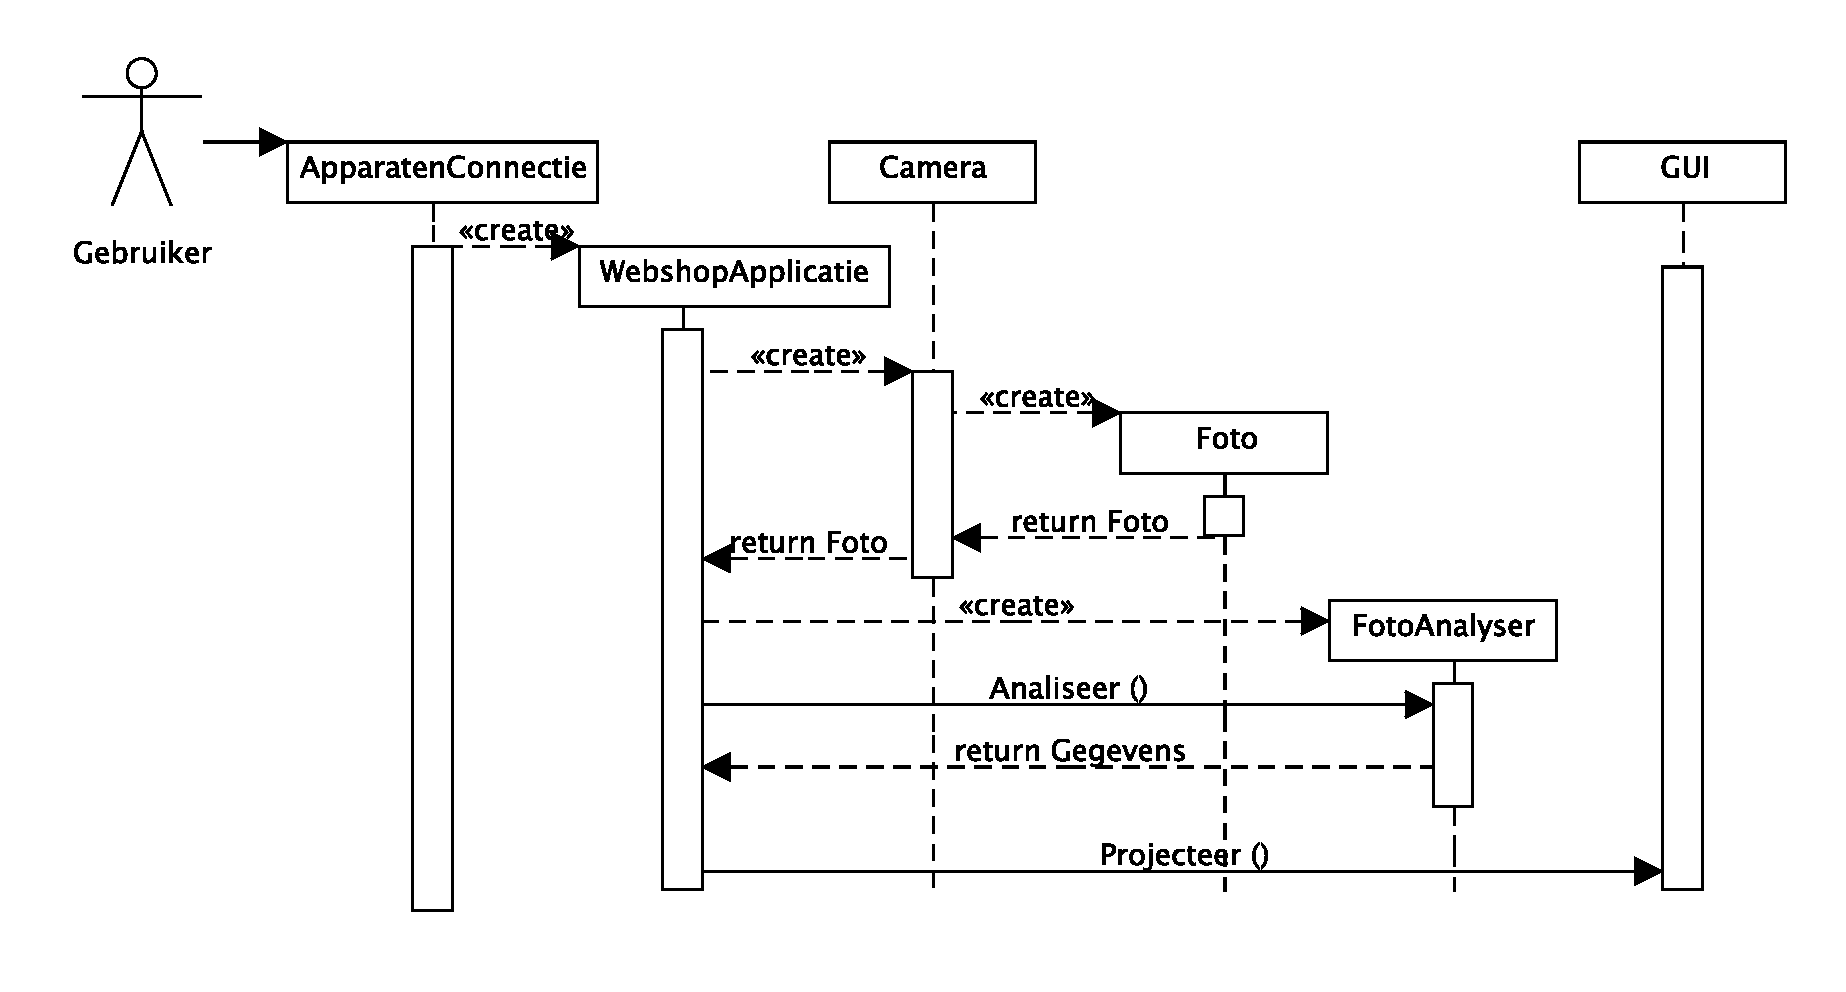
\includegraphics[width=\textwidth]{webshop_sequentie.eps}
    \caption{Interactiediagram webshop}
    \label{graph:graph1}
  \end{center}
\end{figure}

\subsubsection*{Scenario 3: GPS}
\begin{figure}[H]
  \begin{center}
\hspace*{-1.0in}
    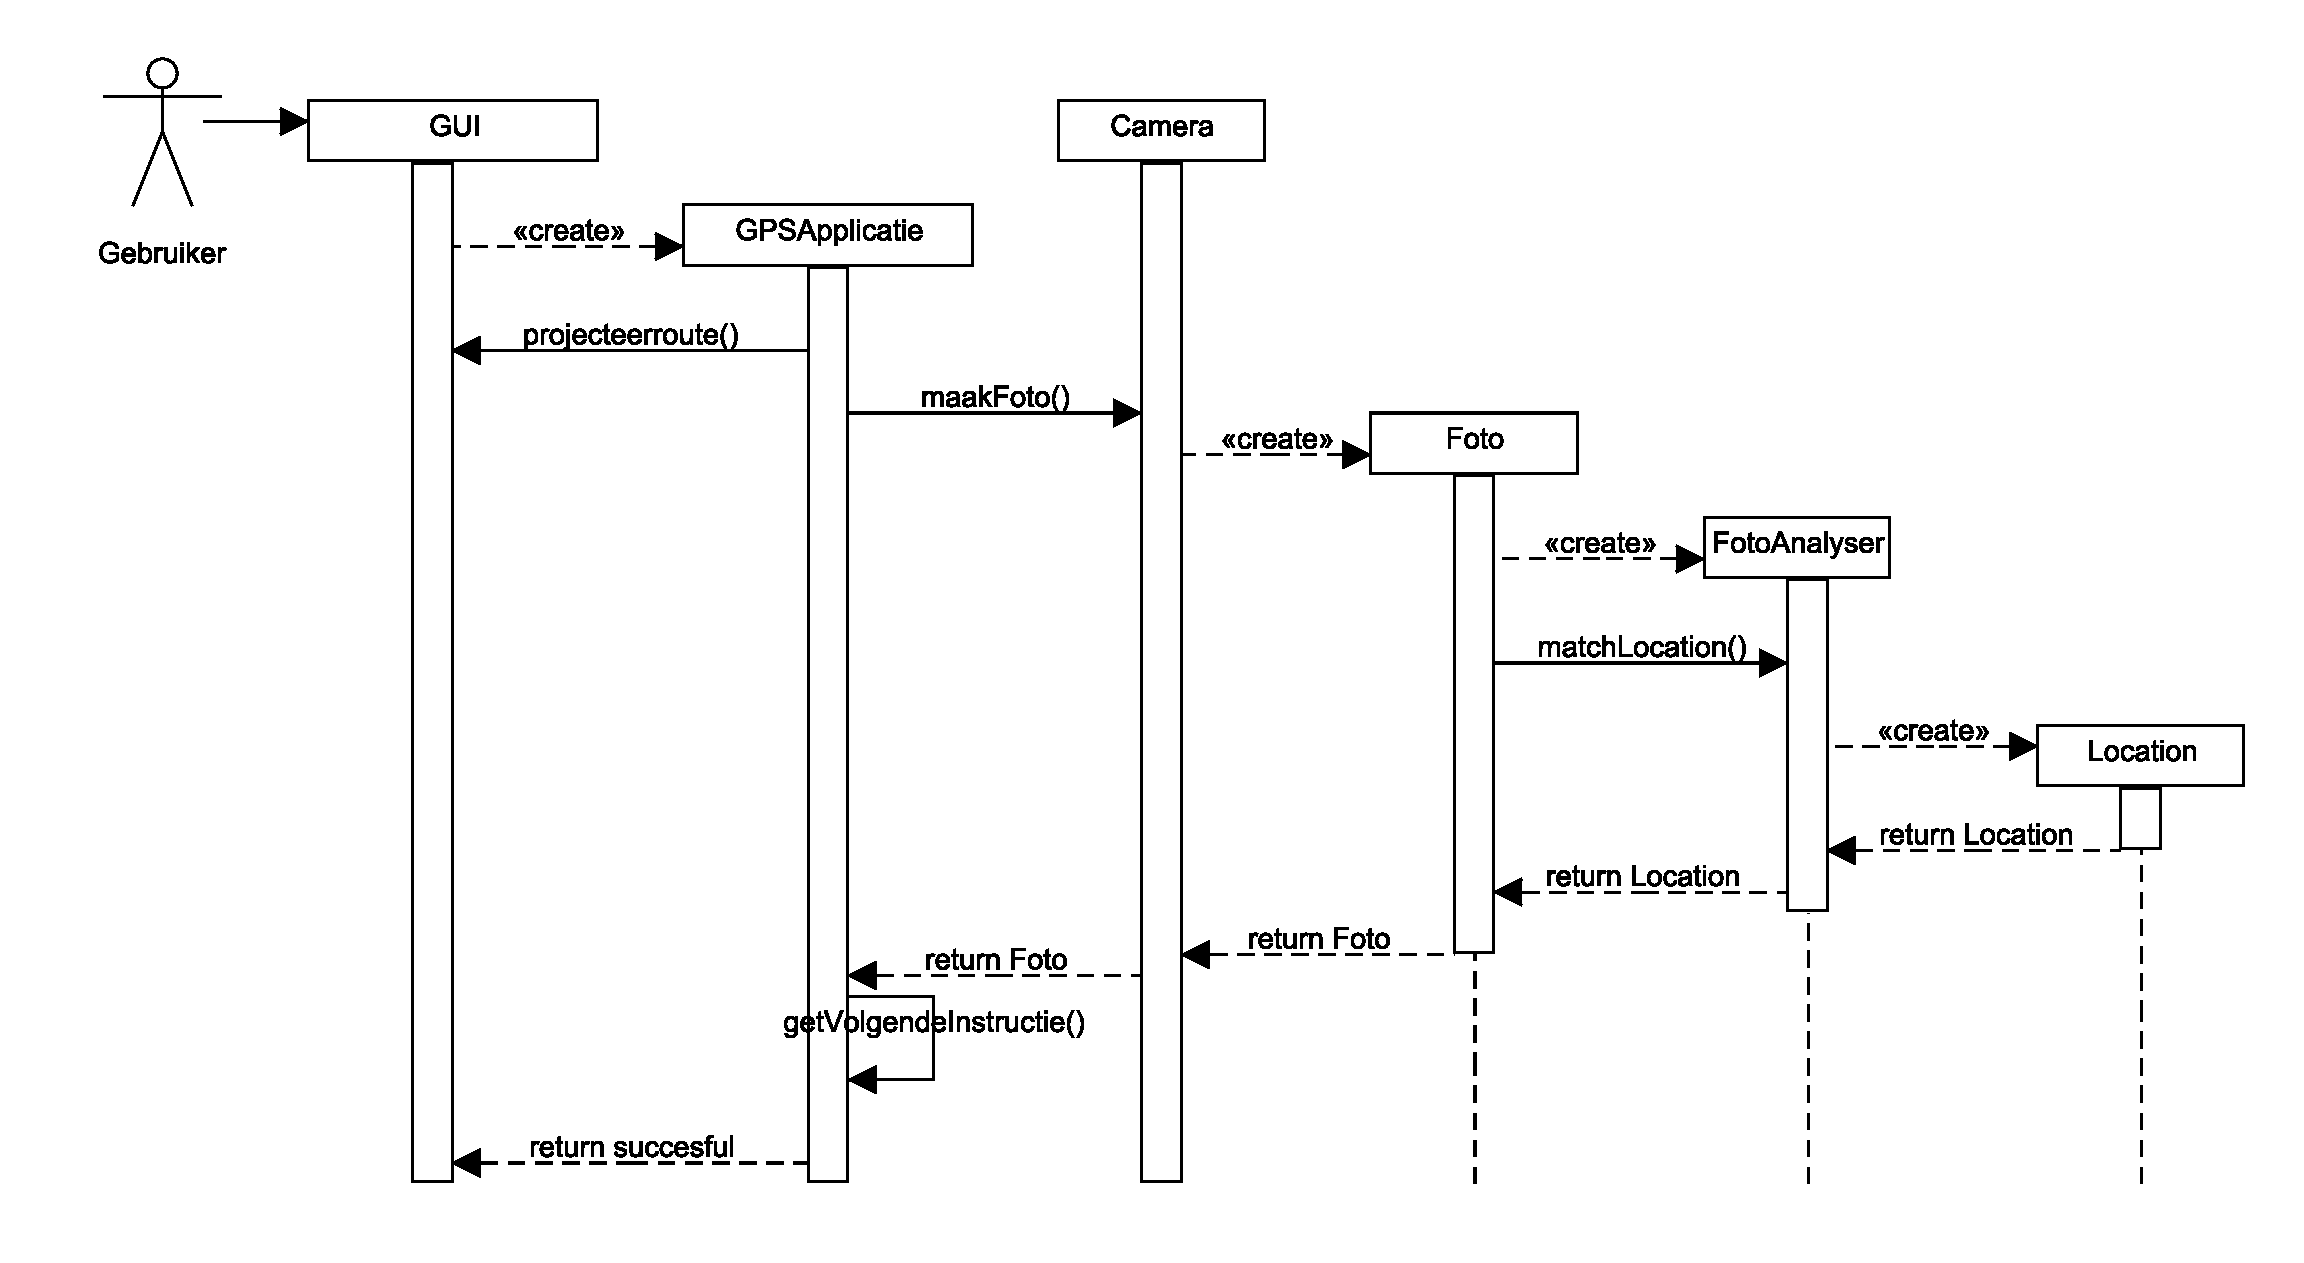
\includegraphics[scale=0.4]{gps_sequentie.eps}
    \caption{Interactiediagram gps}
    \label{graph:graph1}
  \end{center}
\end{figure}

\subsubsection*{Scenario 4: Overlay}
\begin{figure}[H]
  \begin{center}
    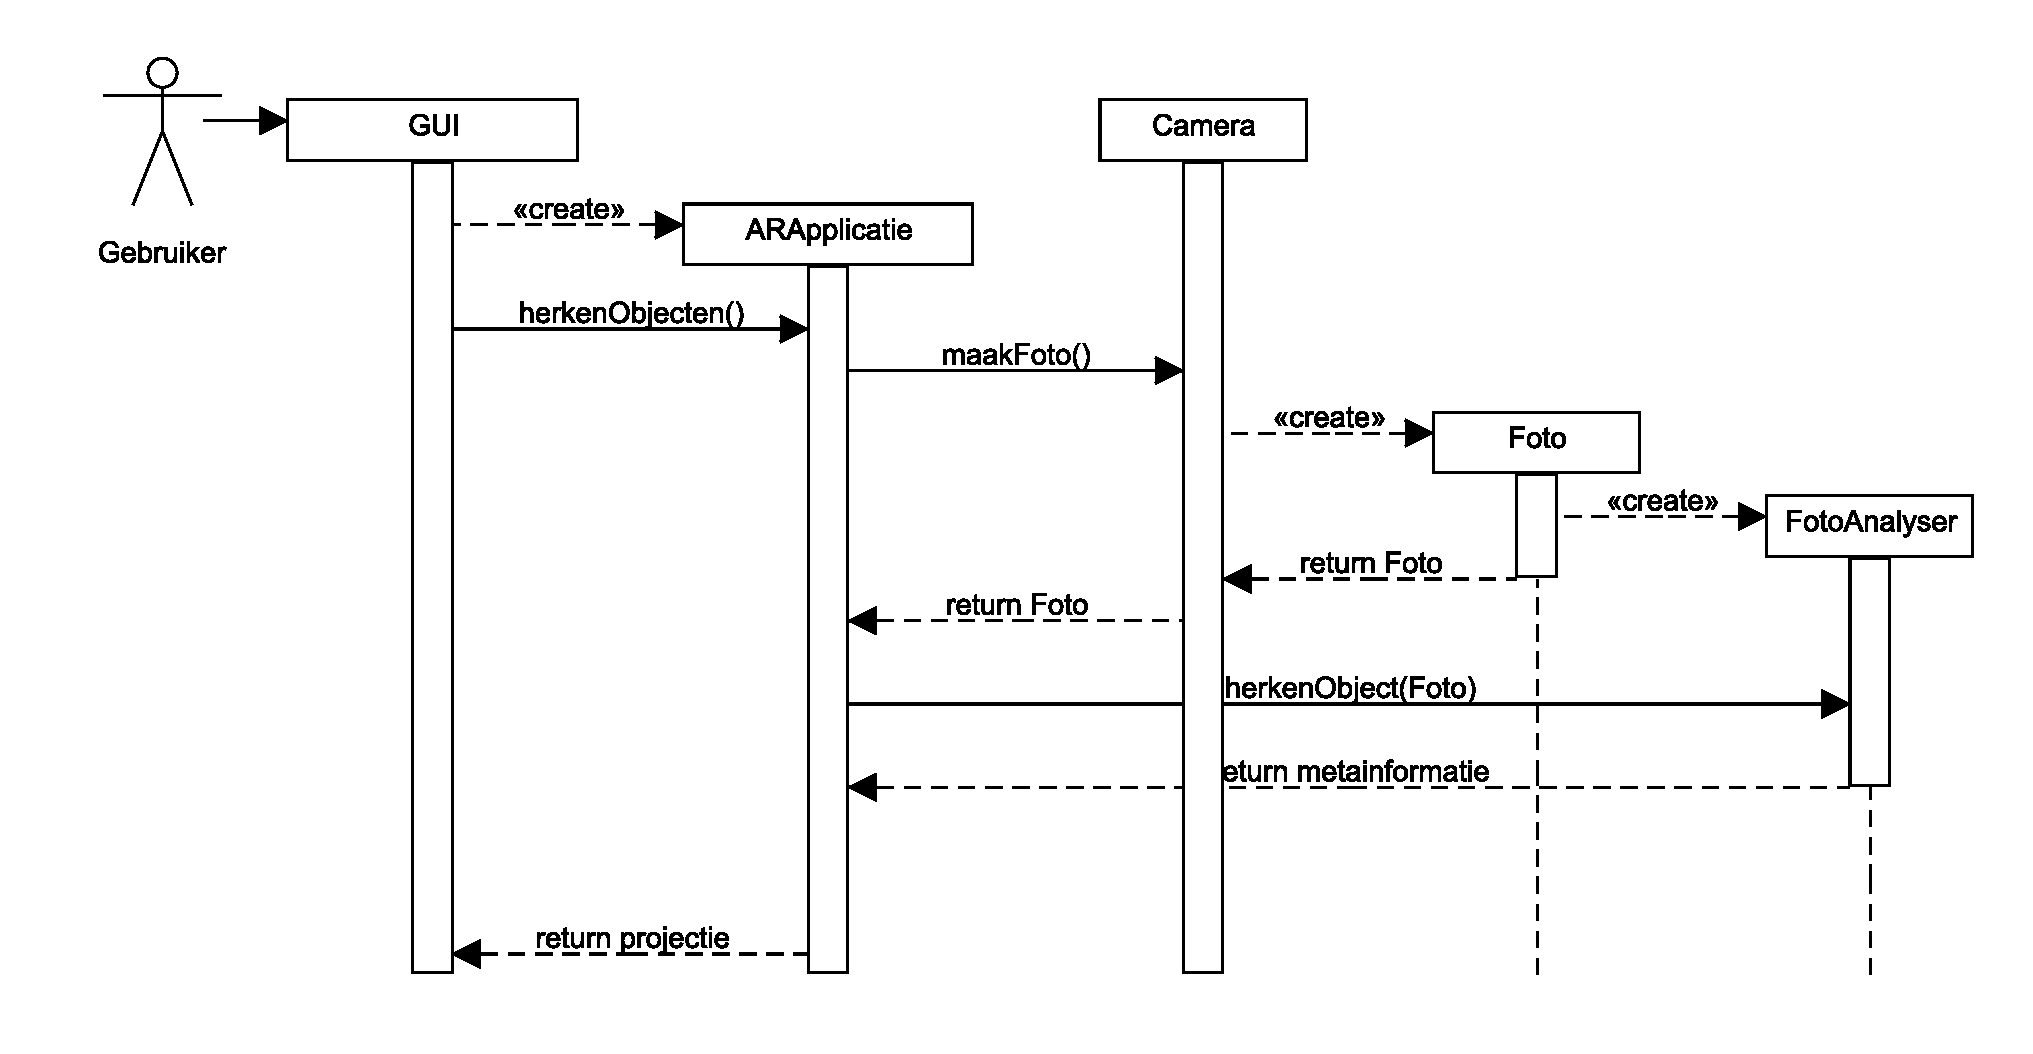
\includegraphics[width=\textwidth]{overlay_sequentie.eps}
    \caption{Interactiediagram overlay}
    \label{graph:graph1}
  \end{center}
\end{figure}


\section{UML klassendiagram}
\begin{figure}[H]
  \begin{center}
    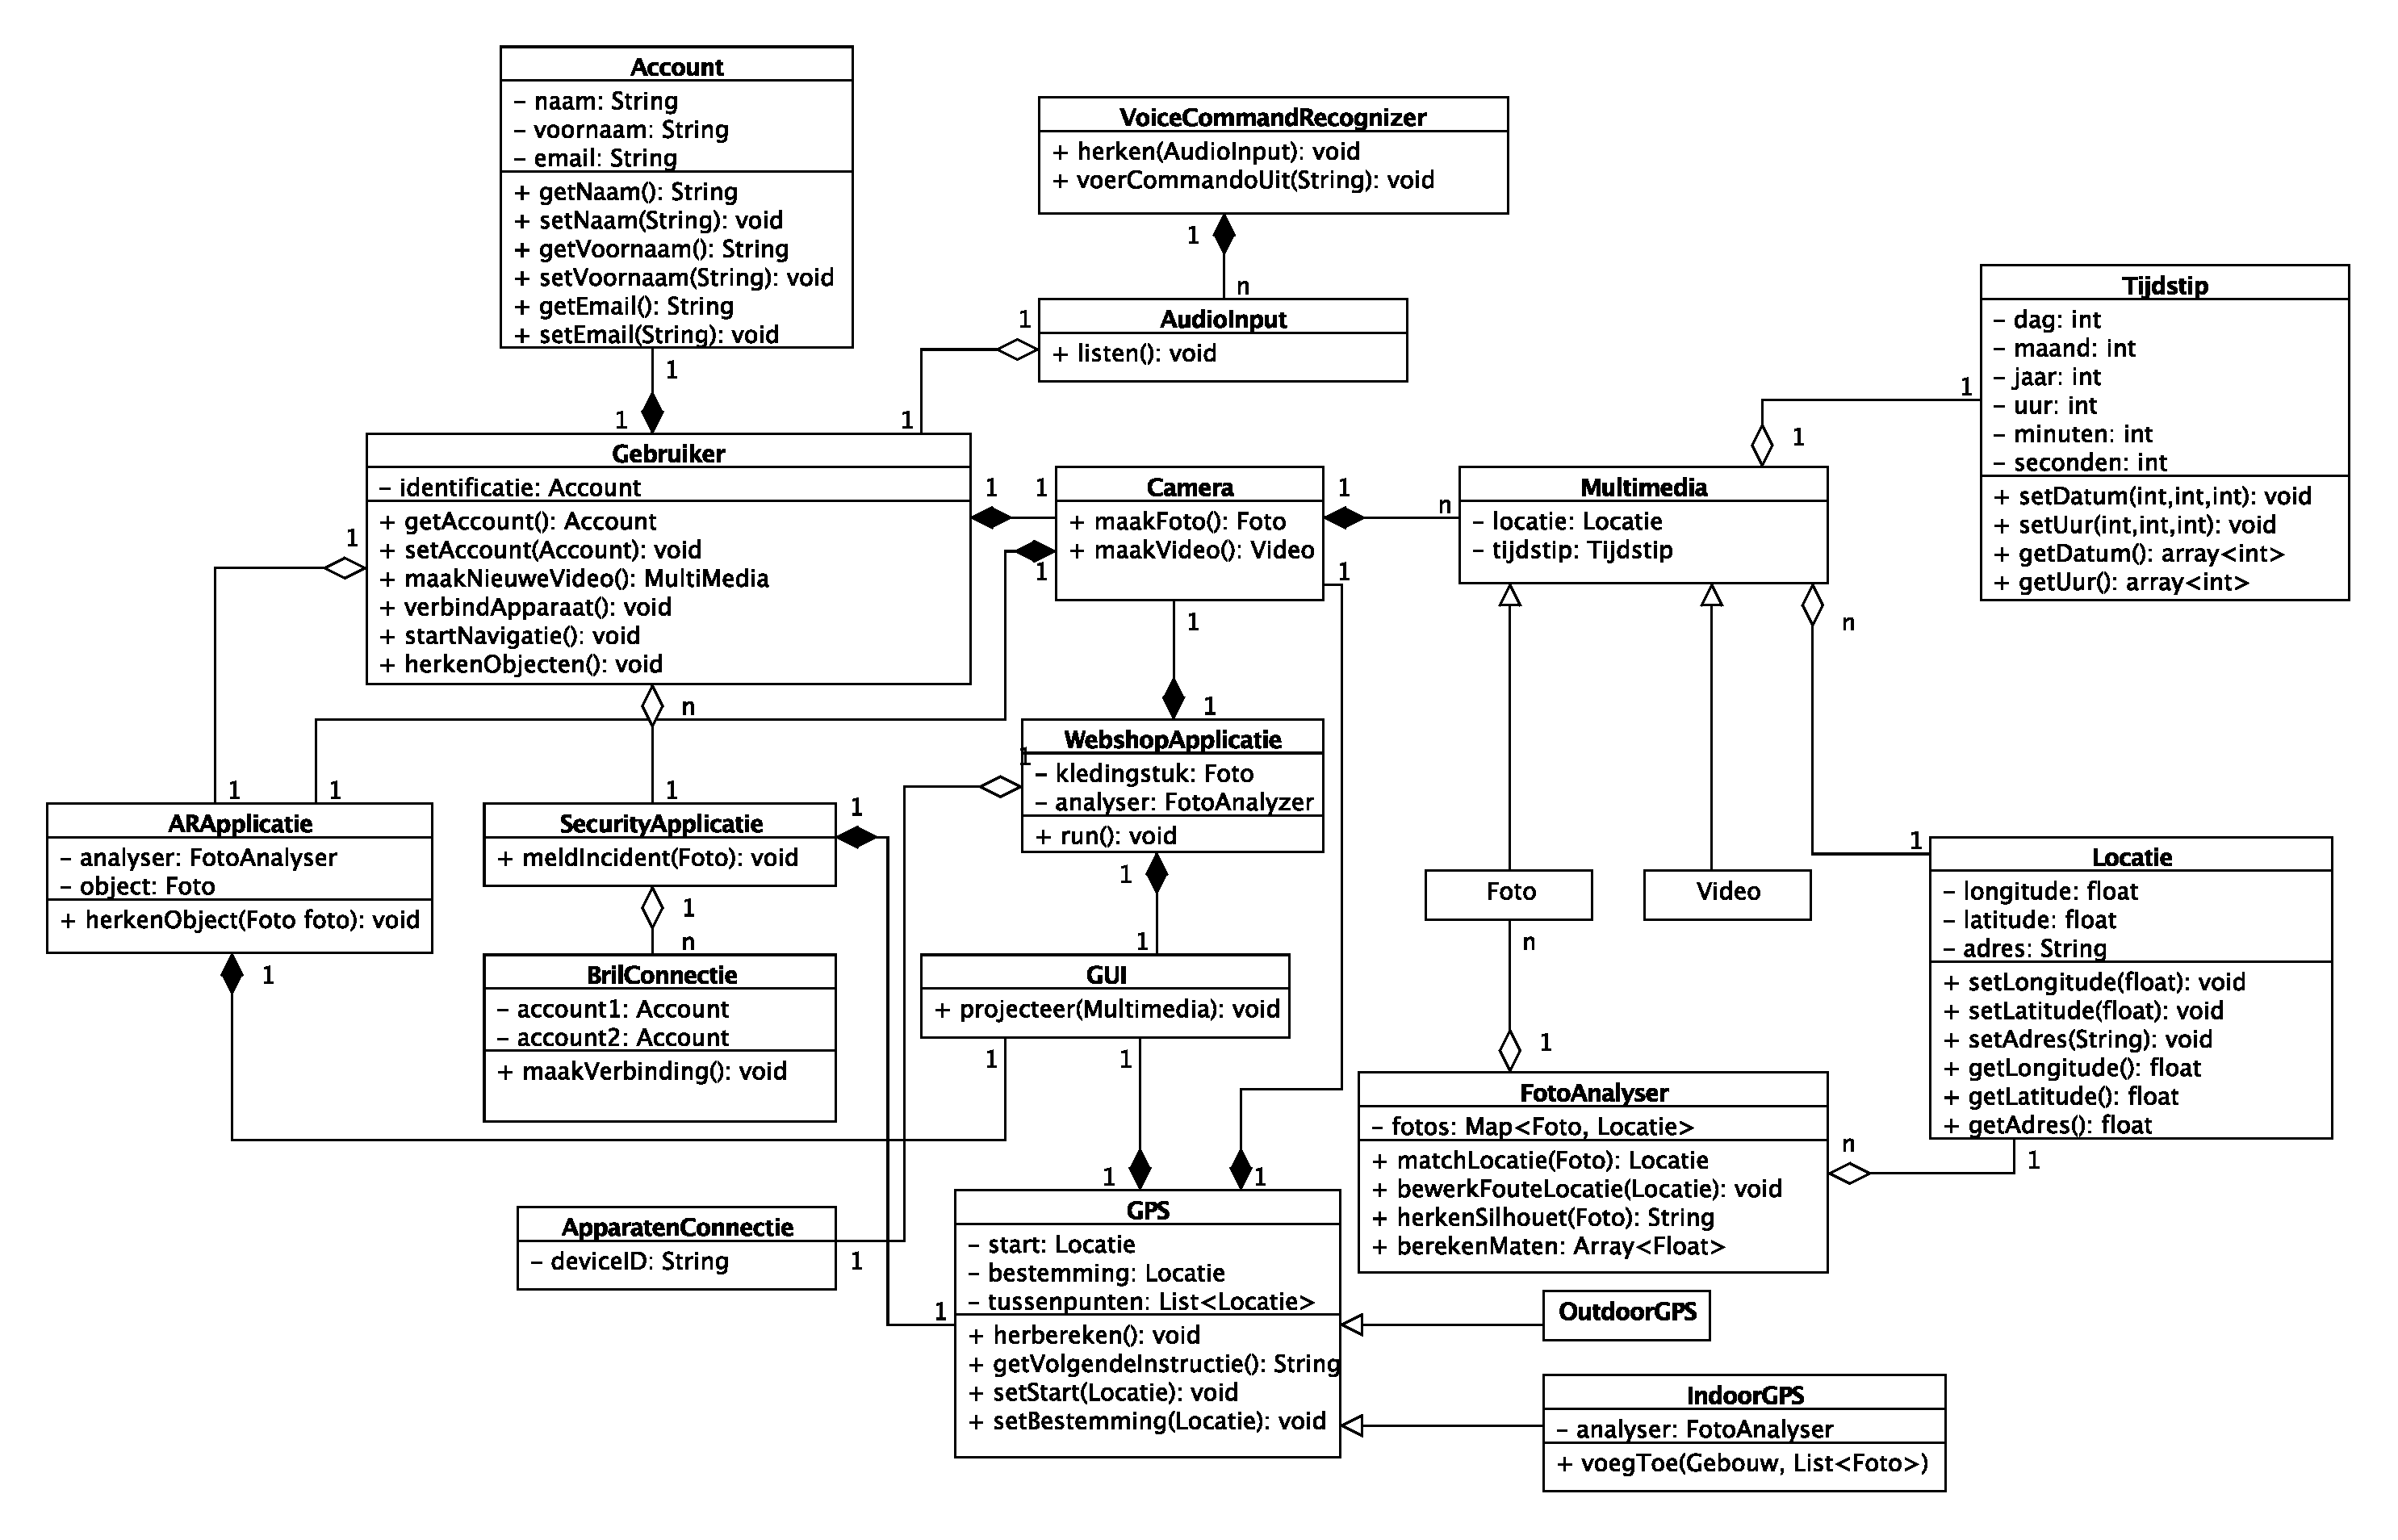
\includegraphics[width=\textwidth]{uml_diagram2.eps}
    \caption{UML diagram}
    \label{graph:graph1}
  \end{center}
\end{figure}


\end{document}